\documentclass[a4paper]{ctexrep}
\usepackage{ctex}
\usepackage{times}
\usepackage{setspace}
\usepackage{fancyhdr}
\usepackage{graphicx}
\usepackage{wrapfig}
\usepackage{array}  
\usepackage{fontspec,xunicode,xltxtra}
\usepackage{titlesec}
\usepackage{titletoc}
\usepackage[titletoc]{appendix}
\usepackage[top=30mm,bottom=30mm,left=20mm,right=20mm]{geometry}
\usepackage{listings}
\usepackage{enumerate}
\usepackage{algorithm}
\usepackage{algorithmicx}
\usepackage{algpseudocode}
\usepackage{color}
\usepackage{appendix}



\definecolor{codegreen}{rgb}{0,0.6,0}
\definecolor{codegray}{rgb}{0.5,0.5,0.5}
\definecolor{codepurple}{rgb}{0.58,0,0.82}
\definecolor{backcolour}{rgb}{0.95,0.95,0.92}




\setmainfont{TeX Gyre Pagella}
\floatname{algorithm}{伪代码}
\renewcommand{\algorithmicrequire}{\textbf{Input:}}
\renewcommand{\algorithmicensure}{\textbf{Output:}}
\newcommand{\numofexp}{七}

%---------------------------------------------------------------------
%	页眉页脚设置
%---------------------------------------------------------------------
\fancypagestyle{plain}{
	\pagestyle{fancy}      %改变章节首页页眉
}

\pagestyle{fancy}
\lhead{\kaishu~TCP/IP课程实验报告~}
\rhead{\kaishu~1030616134~尹达恒~}
\cfoot{\thepage}

%---------------------------------------------------------------------
%	章节标题设置
%---------------------------------------------------------------------
\titleformat{\chapter}{\centering\zihao{-1}\heiti}{实验\numofexp}{1em}{}
\titlespacing{\chapter}{0pt}{*0}{*6}

%---------------------------------------------------------------------
%	目录页设置
%---------------------------------------------------------------------
\titlecontents{chapter}[0em]{\songti\zihao{-4}}{\thecontentslabel\ }{}
{\hspace{.5em}\titlerule*[4pt]{$\cdot$}\contentspage}
\titlecontents{section}[2em]{\vspace{0.1\baselineskip}\songti\zihao{-4}}{\thecontentslabel\ }{}
{\hspace{.5em}\titlerule*[4pt]{$\cdot$}\contentspage}
\titlecontents{subsection}[4em]{\vspace{0.1\baselineskip}\songti\zihao{-4}}{\thecontentslabel\ }{}
{\hspace{.5em}\titlerule*[4pt]{$\cdot$}\contentspage}

\ctexset {
	chapter = {
		name = {实验},
		number = {\numofexp},
	},
	section = {
		number = \arabic{section},
		format = \Large\bfseries,
	},
	subsection = {
		number = \arabic{section}.\arabic{subsection},
	}
}

\begin{document}
%---------------------------------------------------------------------
%	封面设置
%---------------------------------------------------------------------
\begin{titlepage}
	\begin{center}
    
\includegraphics[width=0.9\textwidth]{figure//Njust.png}\\
    \vspace{10mm}
    \textbf{\zihao{2}\kaishu{ 物联网工程学院}}\\[0.8cm]
    \textbf{\zihao{2}\kaishu{ TCP/IP课程实验报告}}\\[3cm]
	\vspace{\fill}
	\setlength{\extrarowheight}{3mm}
	{\songti\zihao{3}	
		\begin{tabular}{rl}
			
			{\makebox[4\ccwd][s]{班\qquad 级:}}& ~\kaishu 物联1601\\
			
			{\makebox[4\ccwd][s]{姓\qquad 名:}}& ~\kaishu 尹达恒 \\ 
			
			{\makebox[4\ccwd][s]{学\qquad 号:}}& ~\kaishu 1030616134 \\ 
			
			{\makebox[4\ccwd][s]{指导老师:}} & ~\kaishu 马君霞\\ 
			
		\end{tabular}
	}\\[2cm]
	\vspace{\fill}
	\zihao{4}
	2018\textasciitilde 2019第一学期\\
	\today
	\end{center}	
\end{titlepage}



%---------------------------------------------------------------------
%  目录页
%---------------------------------------------------------------------
\tableofcontents % 生成目录
%---------------------------------------------------------------------
%  实验一
%---------------------------------------------------------------------
\chapter{基于ICMP协议的ping应用程序综合实验}
\begin{spacing}{1.5}
\songti\zihao{-4}
\lstset{
	language={[Sharp]C},
	numbers=left,numberstyle=\tiny,
	basicstyle=\small\ttfamily,
	stringstyle=\color{codepurple},
	keywordstyle=\color{blue}\bfseries,
	commentstyle=\color{codegreen},
	frame=shadowbox,
	rulesepcolor=\color{codegray}
}
\section{实验目的及要求}
\begin{itemize}
	\item 了解和掌握创建原始套接口的编程方法,注意与创建SOCK\_DGRAM和SOCK\_STREAM类型套接口的区别;
	\item 编写一个基于ICMP协议的Ping应用程序;
	\item 掌握select(),SendEchoRequest(), WaitForEchoReply(), gethostbyname(),sendto()以及recvfrom()等函数的用法。
\end{itemize}
\section{实验环境}
\begin{itemize}
	\item 操作环境:Windows 10;
	\item 编程环境:Visual Studio 2015;
	\item 程序原理:ICMP网络程序设计;
	\item 程序使用Visual C++下的“Win32 Console Application”。
\end{itemize}
\section{实验内容及步骤}
\subsection{基于ICMP协议的ping程序基本原理}
使用SOCK\_RAW套接口编写ping程序测试网络的连通性。ping程序通过生成一个ICMP“回应请求”(cho Request),将其发送到打算查询的目标主机,检测是否可以收到目标主机的应答,以此测试网络的连通性。本实验中的ping程序时实际操作系统中提供的ping程序的简化版,只进行回送测试,测试时需要提供一个目标主机的IP地址信息。需要注意,使用ping程序测试时可达的机器也并不一定能保证一个客户机就一定可以与目标主机的某个进程顺利连接;但若ping程序测试不成功,则可以确定目标机一定与该主机不能建立任何连接。

\subsection{基于ICMP协议的ping程序编写}

\begin{itemize}
	\item 调试环境:Visual Stdio 2015;
	\item 程序名称:TCP7.exe;
	\item 主机IP地址:由系统指定;
	\item 程序功能:启动程序后ping程序通过ICMP协议对输入的IP地址进行4次发送和接收的测试,并显示测试结果;
	\item 命令格式:点分十进制形式的服务器 IP 地址;
	\item 命令举例:192.168.137.1。
\end{itemize}

\subsubsection{ping程序的具体实现步骤}
\begin{enumerate}
	\item 定义IP和ICMP协议头;
	\item 定义回送请求和应答数据包的结构;
	\item 在主程序中初始化Winsock协议栈(使用WSAS()函数);
	\item 在主程序中调用ping函数;
	\item 释放Winsock协议栈。
\end{enumerate}

\subsubsection{ping函数的主要功能}
\begin{enumerate}
	\item 创建一个原始套接口;
	\item 根据主机名查询主机地址;
	\item 输出Ping程序要测试的目标主机地址;
	\item 控制ping程序进行4次发送和接收的测试(发送和接收分别使用SendEchoRequest()和WaitForEchoReply()函数来实现);
	\item 计算传输时间,并输出提示信息;
	\item 关闭原始套接口。
\end{enumerate}

\subsection{本机回环测试}
\begin{itemize}
	\item 测试环境:Visual Studio 2015
	\item 测试步骤:
	\begin{enumerate}
		\item 在一台主机上启动ping程序;
		\item 在ping程序中输入IP地址“127.0.0.1”进行ping操作;
		\item 观察记录实验结果;
		\item 关闭程序。
	\end{enumerate}
\end{itemize}

\subsection{远程互通测试}
\begin{itemize}
	\item 测试环境:Visual Studio 2015
	\item 测试步骤:
	\begin{enumerate}
		\item 将两台主机连入同一个网络;
		\item 分别在两台主机上的命令行窗口输入命令“ipconfig”查看并记录各自的IP地址;
		\item 在一台主机上启动ping程序;
		\item 在ping程序中输入另一台主机的IP地址进行ping操作;
		\item 观察记录实验结果;
		\item 关闭程序;
		\item 在另一台主机上启动ping程序并重复步骤4至步骤6。
	\end{enumerate}
\end{itemize}

\newpage
\section{实验结果}
\subsection{本地回环测试结果}
程序运行结果:图\ref{result}
\begin{figure}[htbp]
	\centering
	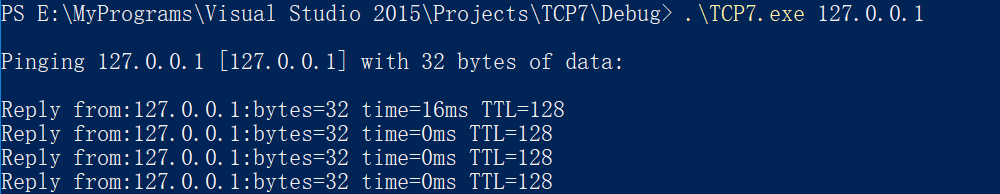
\includegraphics [width=1\textwidth]{figure//res_local.png}
	\caption{本地回环测试结果}\label{result}
\end{figure}

\subsection{远程互通IP记录}
主机1:图\ref{IP1}
\begin{figure}[htbp]
	\centering
	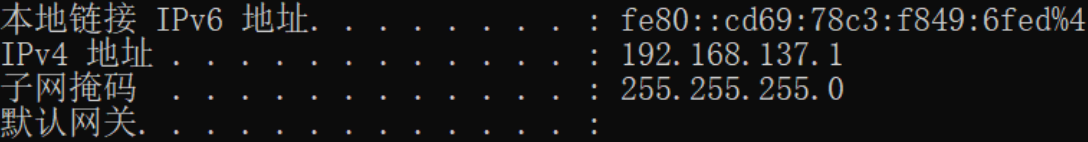
\includegraphics [width=1\textwidth]{figure//IP1.png}
	\caption{主机1IP}\label{IP1}
\end{figure}

主机2:图\ref{IP2}
\begin{figure}[htbp]
	\centering
	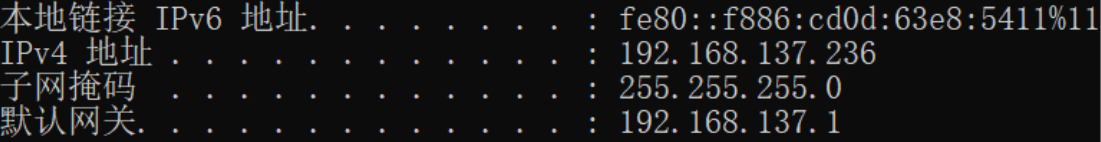
\includegraphics [width=1\textwidth]{figure//IP2.png}
	\caption{主机2IP}\label{IP2}
\end{figure}

\newpage
\subsection{远程互通测试结果1(主机1启动ping)}
主机1:图\ref{remote2}
\begin{figure}[htbp]
	\centering
	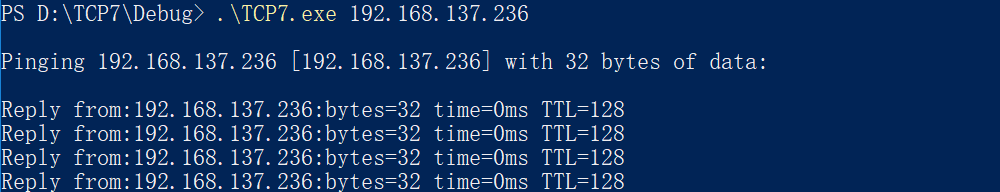
\includegraphics [width=1\textwidth]{figure//res_remote2.png}
	\caption{远程互通测试主机1结果}\label{remote2}
\end{figure}

\subsection{远程互通测试结果2(主机2启动ping)}
主机2:图\ref{remote1}
\begin{figure}[htbp]
	\centering
	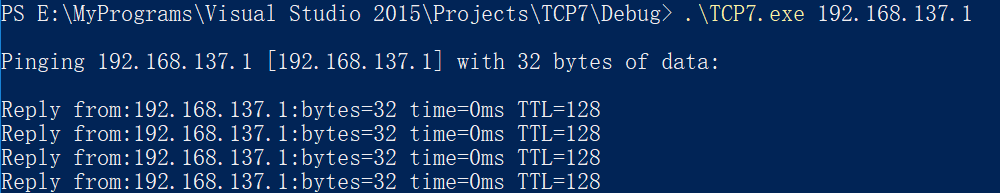
\includegraphics [width=1\textwidth]{figure//res_remote1.png}
	\caption{远程互通测试主机2结果}\label{remote1}
\end{figure}


\end{spacing}
\section{问题及心得}
	\begin{itemize}
		\item 问题:在Visual Stdio中将“\#include "stdafx.h"”放在头文件声明最后时会出现库文件找不到的错误:图\ref{error}
		\begin{figure}[htbp]
			\centering
			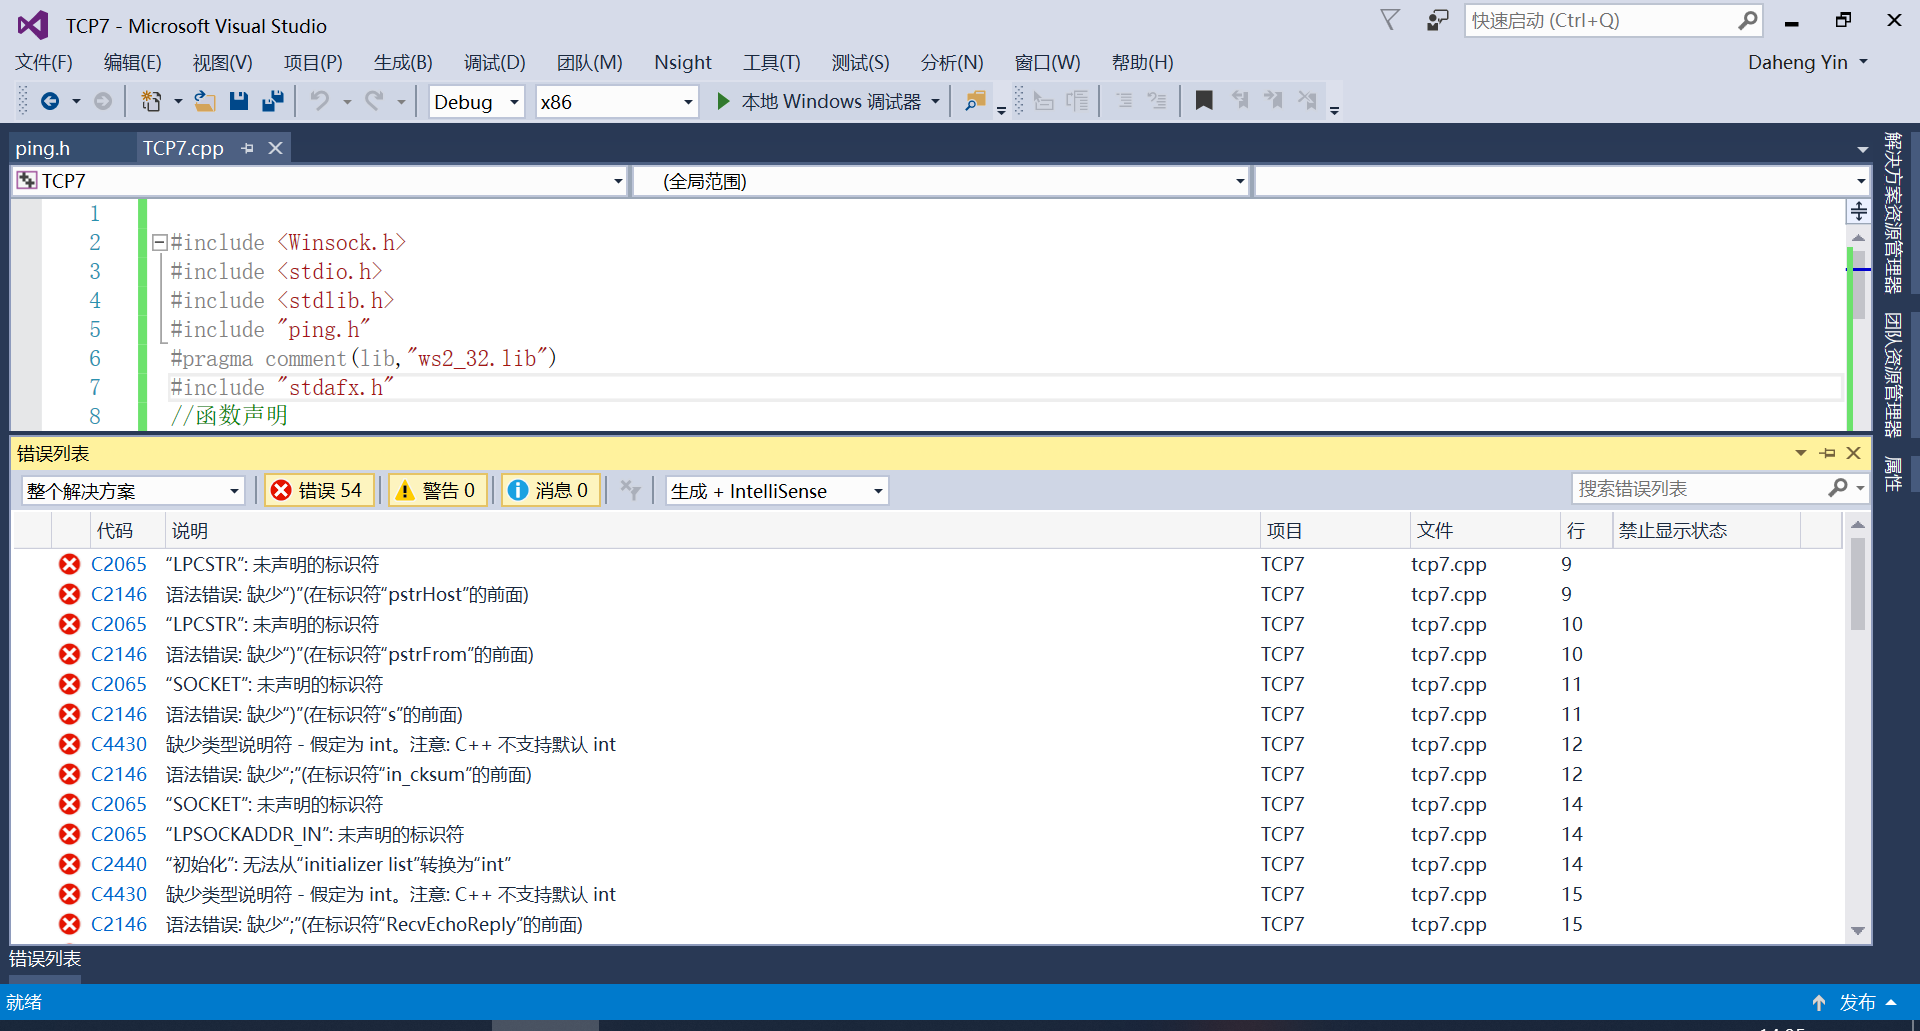
\includegraphics [width=1\textwidth]{figure//err1.png}
			\caption{错误信息}\label{error}
		\end{figure}
	\begin{itemize}
		\item 原因:Visual Stdio自动生成的stdafx.h文件和一些重要的库文件有关,此文件的include声明必须要在其他include声明之前,否则其他include声明就可能出现找不到的情况。
		\item 解决:将“\#include "stdafx.h"”放在文件开头。
	\end{itemize}
		\item 心得:\begin{enumerate}
			\item 实践是检验真理的唯一标准;
			\item 实验是巩固知识的最快捷径;
			\item 掌握了基于ICMP协议ping程序的原理;
			\item 对ICMP协议的理解更加深入;
			\item 精进了代码水平。
		\end{enumerate}
	\end{itemize}
\end{document}